\section*{Questões}
\paragraph{1.}

\subparagraph{a.}
Captura \emph{wireshark} na interface f1/1 de \textsf{R0}, do pedido de IP para interface \textsf{tap0} do \textsf{terminal 1}:

\begin{figure}[h]
\centering
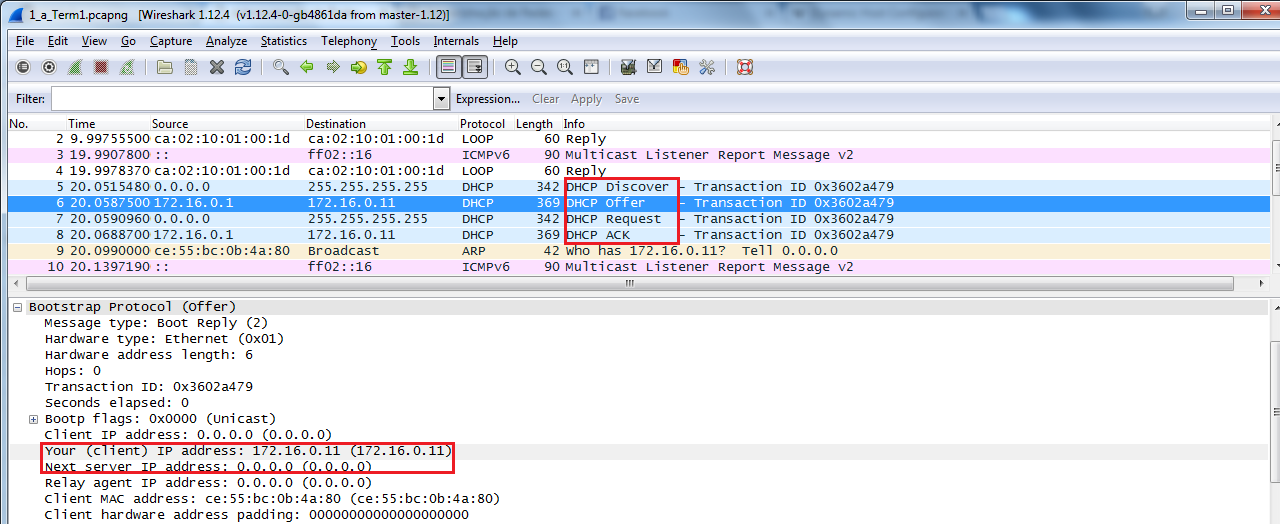
\includegraphics[width=1\textwidth, height=0.3\textheight]{1_a_Terminal1.png}
\label{fig:Term1 DHCP}
\caption{Terminal 1 obtém endereço IP por DHCP.}
\end{figure}

Captura \emph{wireshark} na interface f1/1 de \textsf{R0}, do pedido de IP para interface \textsf{eth0} do \textsf{terminal 2}:

\begin{figure}[h]
\centering
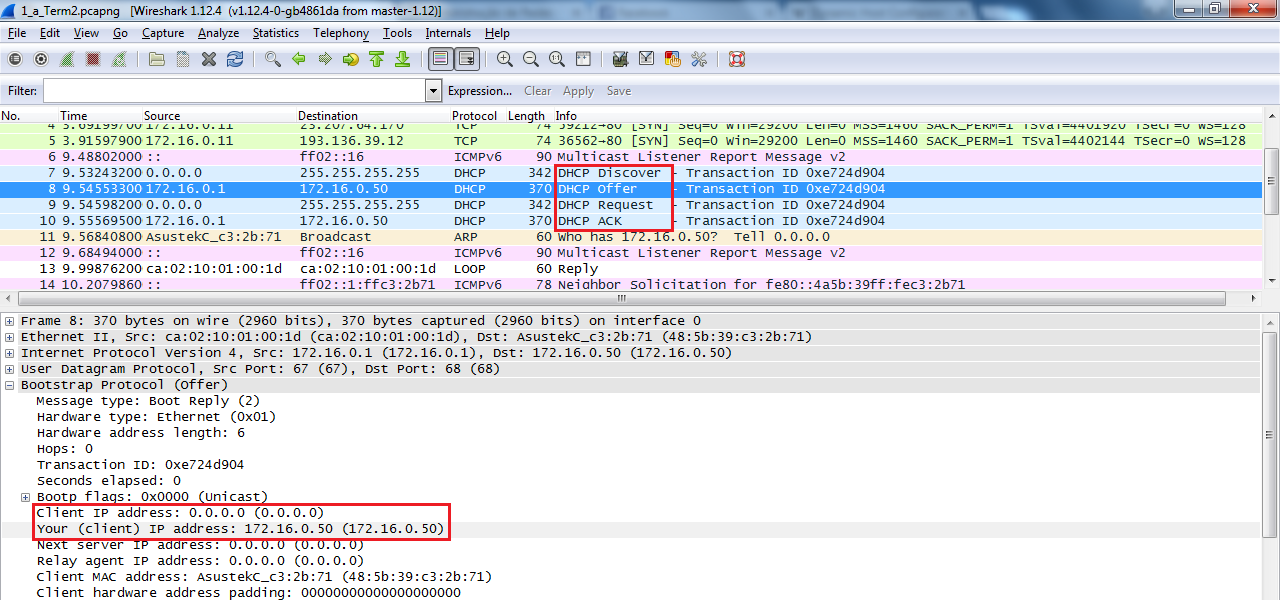
\includegraphics[width=1\textwidth, height=0.33\textheight]{1_a_Terminal2.png}
\label{fig:Term2 DHCP}
\caption{Terminal 2 obtém endereço IP por DHCP.}
\end{figure}


\subparagraph{b.}
Não é possível, a partir das mensagens capturadas, saber qual das duas
máquinas tem um endereço estático (reservado). As mensagens capturadas
mostram uma sequência \textsf{DHCP Discover}, \textsf{Offer}, \textsf{Request} e \textsf{Ack} válida.

No entanto, sabendo que o intervalo da \textsf{pool} do DHCP não contem o IP
atribuído a \textsf{Terminal 1}, podemos concluir que este IP lhe está reservado.

Se tivéssemos observado uma mensagem do tipo \textsf{DHCP Inform}, saberíamos que o
atual cliente tem um IP estático definido por si e apenas pretende
obter informação extra (\textsf{Servidor DNS} e \textsf{Default Gateway}, por
exemplo).


\paragraph{2.}

\begin{verbatim}
Router#debug ip nat detailed
IP NAT detailed debugging is on
Router#
*May  4 15:48:33.015: NAT: Allocated Port for 172.16.0.11 -> 192.168.56.178:
 wanted 39340 got 39340
*May  4 15:48:33.015: NAT*: i: tcp (172.16.0.11, 39340) -> (193.136.39.12, 80)
 [44778]
*May  4 15:48:33.015: NAT*: i: tcp (172.16.0.11, 39340) -> (193.136.39.12, 80)
 [44778]
*May  4 15:48:33.019: NAT*: s=172.16.0.11->192.168.56.178, d=193.136.39.12
 [44778]
*May  4 15:48:33.051: NAT*: o: tcp (193.136.39.12, 80) -> (192.168.56.178,
 39340) [0]
*May  4 15:48:33.051: NAT*: s=193.136.39.12, d=192.168.56.178->172.16.0.11 [0]
*May  4 15:48:33.059: NAT*: i: tcp (172.16.0.11, 39340) -> (193.136.39.12, 80)
 [44779]
*May  4 15:48:33.059: NAT*: s=172.16.0.11->192.168.56.178, d=193.136.39.12
 [44779]
*May  4 15:48:33.059: NAT*: i: tcp (172.16.0.11, 39340) -> (193.136.39.12, 80)
 [44780]
*May  4 15:48:33.059: NAT*: s=172.16.0.11->192.168.56.178, d=193.136.39.12
 [44780]
*May  4 15:48:33.075: NAT*: o: tcp (193.136.39.12, 80) -> (192.168.56.178,
 39340) [32364]
*May  4 15:48:33.075: NAT*: s=193.136.39.12, d=192.168.56.178->172.16.0.11
 [32364]
*May  4 15:48:33.291: NAT*: o: tcp (193.136.39.12, 80) -> (192.168.56.178,
 39340) [32365]
*May  4 15:48:33.291: NAT*: s=193.136.39.12, d=192.168.56.178->172.16.0.11
 [32365]
*May  4 15:48:33.291: NAT*: o: tcp (193.136.39.12, 80) -> (192.168.56.178,
 39340) [32366]
*May  4 15:48:33.291: NAT*: s=193.136.39.12, d=192.168.56.178->172.16.0.11
 [32366]
*May  4 15:48:33.295: NAT*: o: tcp (193.136.39.12, 80) -> (192.168.56.178,
 39340) [32367]
*May  4 15:48:33.295: NAT*: s=193.136.39.12, d=192.168.56.178->172.16.0.11
 [32367]
*May  4 15:48:33.295: NAT*: o: tcp (193.136.39.12, 80) -> (192.168.56.178,
 39340) [32368]
*May  4 15:48:33.299: NAT*: s=193.136.39.12, d=192.168.56.178->172.16.0.11
 [32368]
*May  4 15:48:33.323: NAT*: i: tcp (172.16.0.11, 39340) -> (193.136.39.12, 80)
 [44781]
*May  4 15:48:33.323: NAT*: s=172.16.0.11->192.168.56.178, d=193.136.39.12
 [44781]
*May  4 15:48:33.323: NAT*: i: tcp (172.16.0.11, 39340) -> (193.136.39.12, 80)
 [44782]
*May  4 15:48:33.323: NAT*: s=172.16.0.11->192.168.56.178, d=193.136.39.12
 [44782]
*May  4 15:48:33.323: NAT*: i: tcp (172.16.0.11, 39340) -> (193.136.39.12, 80)
 [44783]
*May  4 15:48:33.323: NAT*: s=172.16.0.11->192.168.56.178, d=193.136.39.12
 [44783]
*May  4 15:48:33.335: NAT*: o: tcp (193.136.39.12, 80) -> (192.168.56.178,
 39340) [32368]
*May  4 15:48:33.335: NAT*: s=193.136.39.12, d=192.168.56.178->172.16.0.11
 [32368]
*May  4 15:48:33.335: NAT*: o: tcp (193.136.39.12, 80) -> (192.168.56.178,
 39340) [32369]

...
\end{verbatim}

O trabalho do NAT é realizar uma tradução de endereços de rede privado (no nosso caso, \textsf{172.16.0.11}), em um endereço público (\textsf{192.168.56.178}). Isto permite  que um computador de uma rede interna (privada) tenha acesso ao exterior, rede pública.


\paragraph{3.}
Quando usamos o comando \texttt{clear ip nat translation *}, deixamos de receber os \textsf{"hello"}.\\
"Quando usamos NAT com tradução de portas, os fluxos de pacotes passam de \emph{connectionless} para \emph{connection-oriented}", ou seja, o \textsf{\emph{router} Cisco} tem uma tabela de traduções de \textsf{IPs} internos para externos e vice-versa, (mantém informação sobre as conexões).\\
O comando acima permite-nos limpar todas as traduções dinâmicas da tabela de tradução do \emph{router}, perdendo a conexão, uma vez que apagamos toda a informação da tabela, voltando assim para \emph{connectionless}, sendo por esta razão que deixamos de receber os \textsf{"hello"}.


\paragraph{4.}

\subparagraph{a.}
\begin{verbatim}
[root@Labs5616 ar]# ssh 192.168.56.20
\end{verbatim}


\subparagraph{b.}
Os \textsc{IPs} privados numa rede local não são acessíveis fora da rede, a partir da internet. O \emph{port forwarding} serve para permitir que uma dada máquina chegue (usando NAT) a uma porta de um IP privado, mesmo fora dessa rede, este atribui uma porta a um dispositivo.\\
Usando uma porta não-standard quando temos mais que um terminal numa sub-rede, teríamos de usar portas diferentes para aceder de uma rede externa a uma rede interna, neste caso, ao \textsf{\emph{router} Linux} e ao \textsf{Terminal 2}.

\newpage

\paragraph{5.}

\subparagraph{a.}

Justifique o insucesso deste procedimento. ????


\subparagraph{b.}
\begin{verbatim}
[root@Labs5616 Trab3]# iptables -t nat -A PREROUTING -p tcp -i enp0s7 
  -d 192.168.56.26 --dport 21 -j DNAT --to 10.0.0.22:21

[root@Labs5616 Trab3]# iptables-save
# Generated by iptables-save v1.4.21 on Wed May  4 17:54:11 2016
*nat
:PREROUTING ACCEPT [5:626]
:INPUT ACCEPT [1:328]
:OUTPUT ACCEPT [16:1194]
:POSTROUTING ACCEPT [3:234]
-A PREROUTING -d 192.168.56.26/32 -i enp0s7 -p tcp -m tcp --dport 21 
  -j DNAT --to-destination 10.0.0.22:21
-A POSTROUTING -o enp0s7 -j MASQUERADE
COMMIT
# Completed on Wed May  4 17:54:11 2016
# Generated by iptables-save v1.4.21 on Wed May  4 17:54:11 2016
*filter
:INPUT ACCEPT [21329:24200039]
:FORWARD ACCEPT [99770:70460139]
:OUTPUT ACCEPT [13750:876654]
COMMIT
# Completed on Wed May  4 17:54:11 2016
[root@Labs5616 Trab3]# 
\end{verbatim}


\subparagraph{c.}
Captura \emph{wireshark} na interface \textsf{enp0s7 - 192.168.56.26} do \textsf{Router Linux}:

\begin{figure}[h]
\centering
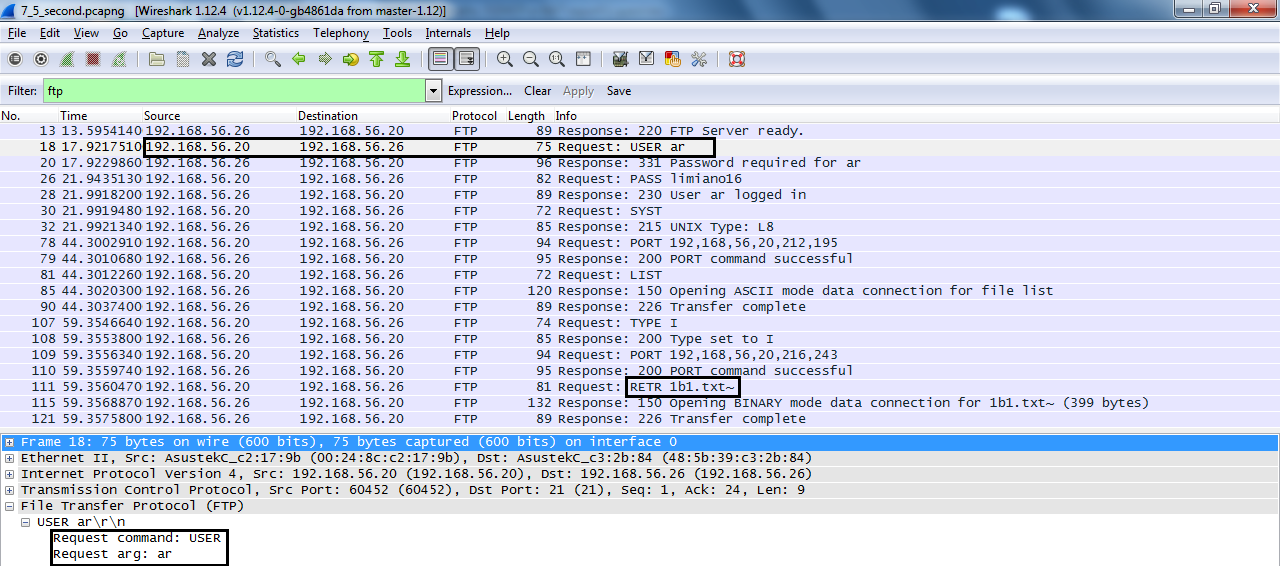
\includegraphics[width=1\textwidth, height=0.3\textheight]{5_b-enp0s7.png}
\label{fig:enp0s7}
\caption{Captura \emph{wireshark} na interface \textsf{192.168.56.26}.}
\end{figure}

Captura \emph{wireshark} na interface \textsf{enp1s6 - 10.0.0.1} do \textsf{Router Linux}:

\begin{figure}[h]
\centering
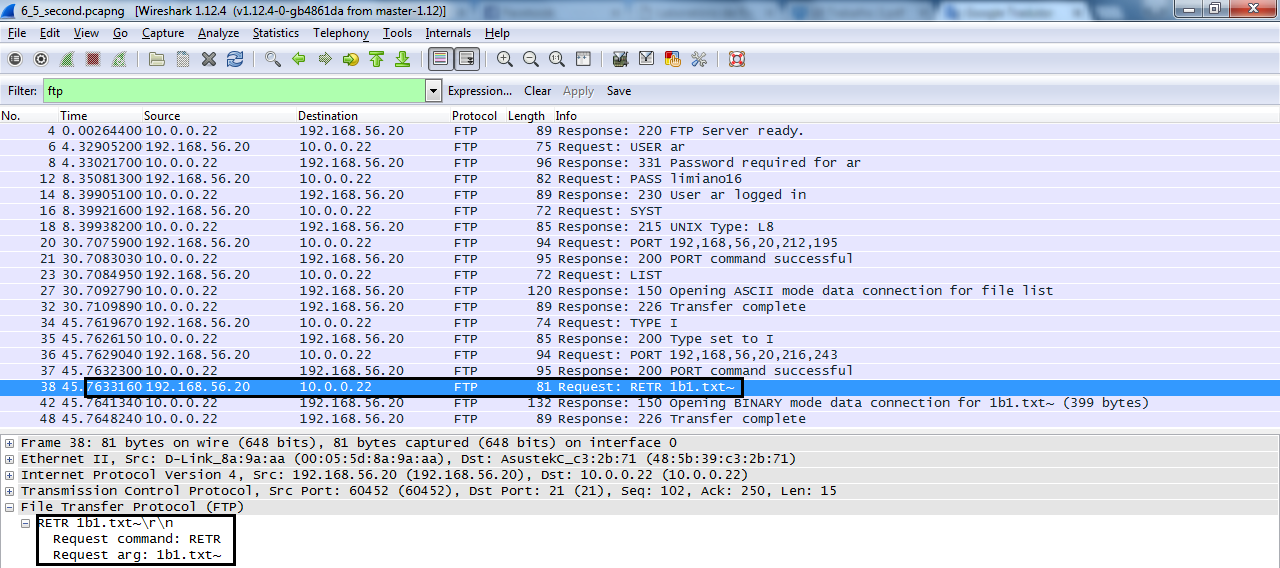
\includegraphics[width=1\textwidth, height=0.3\textheight]{5_b-enp1s6.png}
\label{fig:enp1s6}
\caption{Captura \emph{wireshark} na interface \textsf{10.0.0.1}.}
\end{figure}

Com \emph{port-forwarding} (entrada estática na tabela NAT) todos os
pacotes para um IP+porta exterior (inside global) são sempre
traduzidos para um IP+porta interior (inside local) o que significa
que quando o \textsf{Terminal 1} envia pacotes (ftp) à porta 21 do 
\textsf{\emph{router} Linux}, estes estão a ser encaminhados para o \textsf{10.0.0.22:21} (\textsc{Terminal 2}), destino inacessível pelo 
\textbf{Terminal 1} diretamente. O \textsf{\emph{router} Linux} 
reescreve os cabeçalhos dos pacotes com destino a \textsf{192.168.56.26:21} 
e origem \textsf{IP:PORT} e encaminha-os para \textsf{10.0.0.22} 
desta vez com cabeçalho destino \textsf{10.0.0.22} e a mesma origem.


Como \textsf{10.0.0.22} responde a \textsf{IP:PORT} (\textsf{192.168.56.20}) 
e sabe a rota para esse destino, a comunicação é bem sucedida.


\subparagraph{d.}

\begin{figure}[h]
\centering
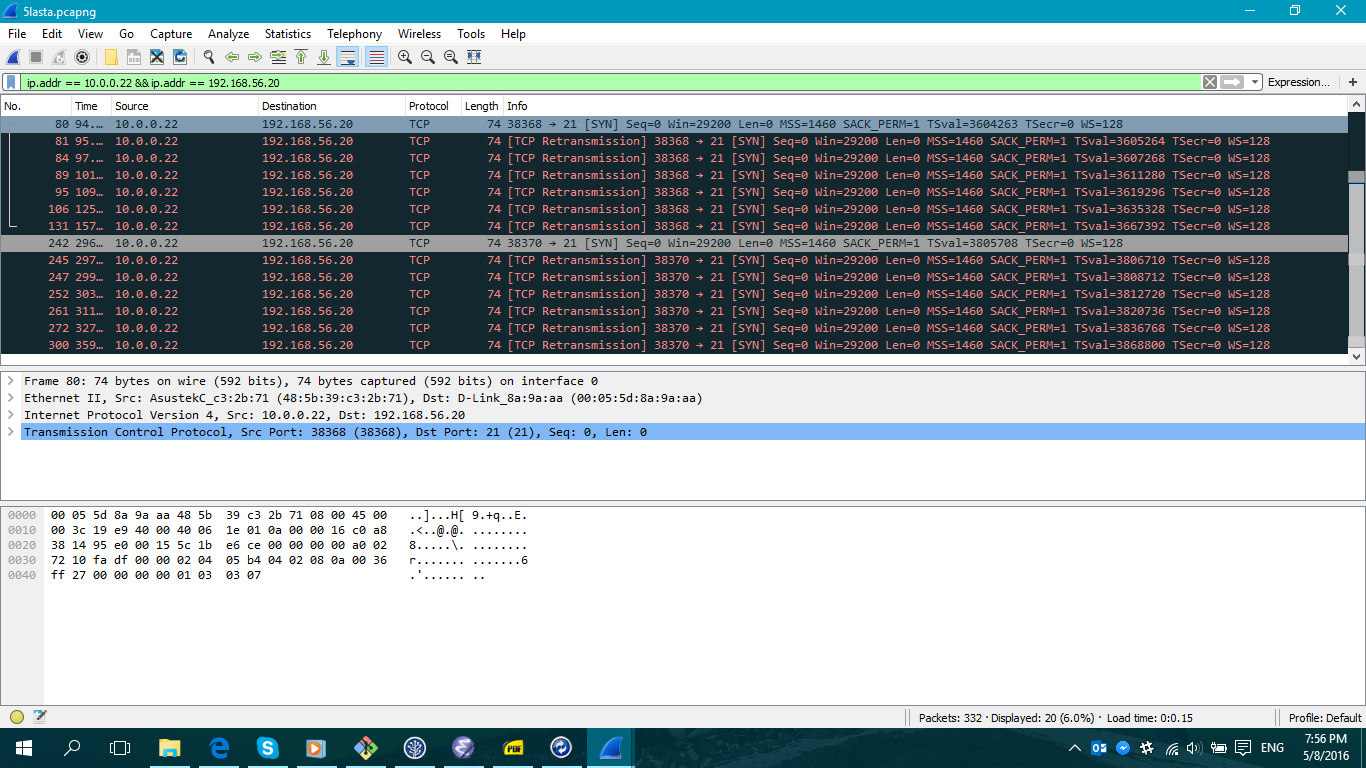
\includegraphics[width=0.9\textwidth, height=0.3\textheight]{5d.png}
\label{fig:5d}
\caption{Captura \emph{wireshark} nas interfaces de \textsf{Router Linux}.}
\end{figure}

A conexão não é bem sucedida pois o \textsf{\emph{router} Linux} limita-se 
a retransmitir os pacotes do \textsf{Terminal 2} para o \textsf{Terminal 1} 
mantendo os cabeçalhos nos pacotes. Como \textsf{Terminal 1} não sabe a rota 
para o endereço do \textsf{Terminal 2} escrito no cabeçalho (\textsf{10.0.0.22}), 
a conexão não é bidirecional, logo não é bem sucedida.

\subparagraph{e.}

\begin{figure}[h]
\centering
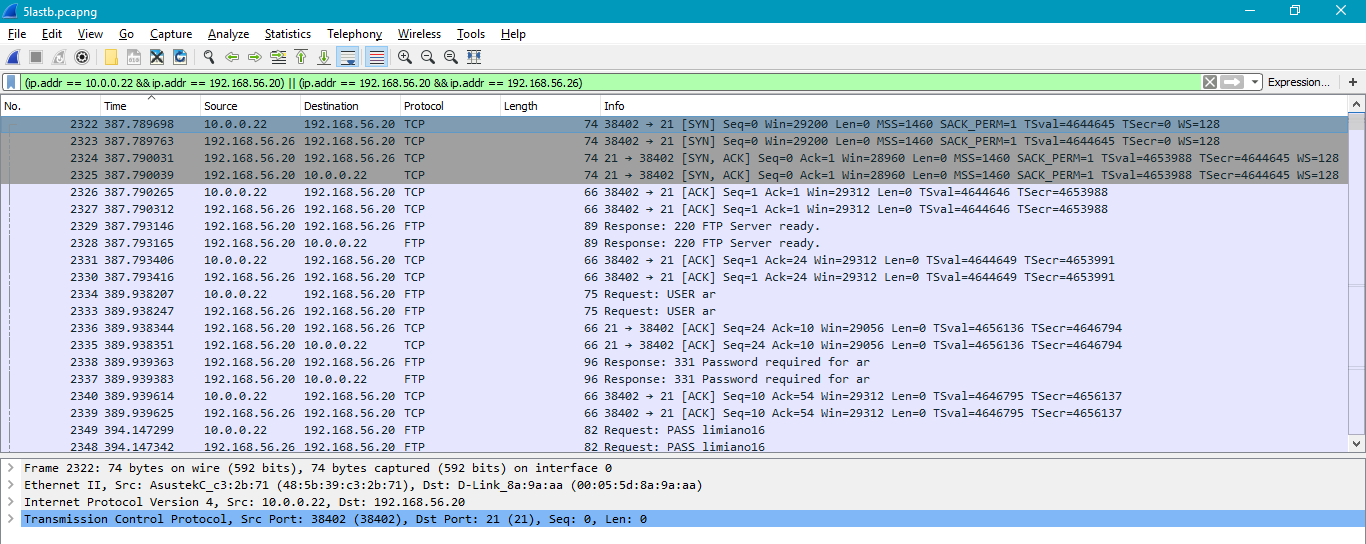
\includegraphics[width=0.9\textwidth, height=0.3\textheight]{5e.png}
\label{fig:5e}
\caption{Captura \emph{wireshark} nas interfaces de \textsf{Router Linux}.}
\end{figure}

Com a instalação do módulo \textsf{nf\_nat\_ftp}, o \textsf{\emph{router} Linux}
reescreve o cabeçalho dos pacotes que por si passam, permitindo que o
\textsf{Terminal 1} responda ao \textsf{Terminal 2}, através do 
\textsf{\emph{router} Linux} e uma porta dedicada para esse efeito 
(neste caso \textsf{38402} é a \textsf{Dst port} no \textsf{Terminal 1} e
no \textsf{\emph{router} Linux}).

Como podemos ver pelo dump do Wireshark ordenado temporalmente, do 
\textsf{Terminal 2} para o \textsf{Terminal 1} altera-se o campo 
\emph{source} para o \textsf{Terminal 1} conseguir responder; do 
\textsf{Terminal 1} para o \textsf{Terminal 2} altera-se o campo 
\emph{destination} para o pacote ser aceite pelo \textsf{Terminal 2}.
